\colorlet{species background color}{black!15}
\tikzset{
    x={1pt},
    y={-1pt},
    species border/.style={
        line width={1pt},
        shorten <={-1pt / 2 + 0.05pt},
        shorten >={-1pt / 2 + 0.05pt},
    },
    species background/.style={
        fill=species background color,
        draw=species background color,
        line width={1pt},
        rounded corners,
    },
    species label/.style={
        font=\bfseries,
        midway,
        anchor=west,
        align=left,
        xshift=10,
    },
    branch/.style={
        draw={#1},
        line width={0.5pt},
    },
    transfer branch/.style={
        branch={#1},
        -Stealth,
    },
    loss/.style={
        draw={#1}, cross out, thick,
        line width={0.5pt},
        inner sep=0pt,
        outer sep=0pt,
        minimum width={3},
        minimum height={3},
    },
    extant gene/.style 2 args={
        circle, fill={#1},
        outer sep=0pt, inner sep=0pt,
        minimum size={3},
        label={
            [font={\color{#1}},
                align=justify,
                inner xsep=4pt, inner ysep=0pt,
                outer xsep=0pt, outer ysep=0pt]
            right:#2
        },
    },
    extant gene/.default={black}{},
    branch node/.style={
        draw={#1}, fill={species background color!50!white},
        align=center,
        font={\color{#1}},
        outer sep=0pt, inner xsep=0pt, inner ysep=2pt,
        line width={0.5pt},
    },
    branch node/.default={black},
    speciation/.style={
        branch node={#1}, rectangle, rounded corners,
        inner xsep=4pt,
        minimum width={8},
        minimum height={8},
    },
    duplication/.style={
        branch node={#1}, rectangle,
        inner xsep=4pt,
        minimum width={8},
        minimum height={8},
    },
    horizontal gene transfer/.style={
        branch node={#1}, chamfered rectangle,
        chamfered rectangle sep={8 / 2.4},
        inner xsep=2pt,
        inner ysep=-1pt,
        minimum width={8},
        minimum height={8},
    },
}
\definecolor{reccolor0}{HTML}{000000}
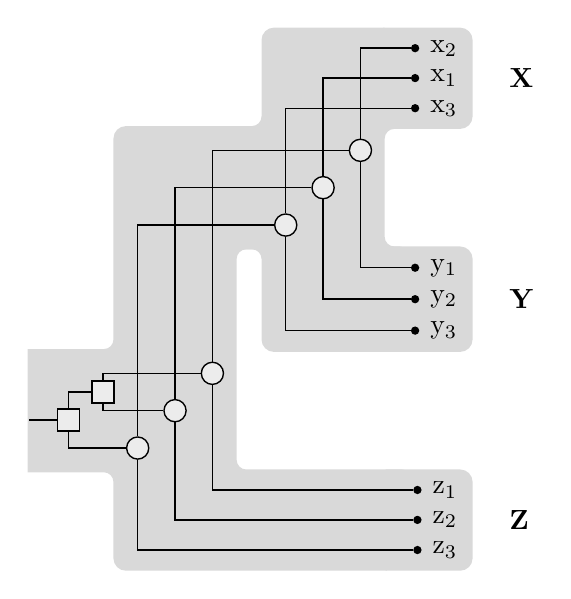
\begin{tikzpicture}
% background
\path[species background] (74.5,35.56989) -- (31.0,35.56989) -- (31.0,116.14986) [sharp corners] -- (0,116.14986) -- (0,159.64986) [rounded corners] -- (31.0,159.64986) -- (31.0,195.21974999999998) [sharp corners] -- (128.84,195.21974999999998) [rounded corners] -- (138.84,159.64986) -- (74.5,159.64986) -- (74.5,79.06989) [sharp corners] -- (84.5,79.06989) -- cycle;
\path[species background] (128.0,0) -- (84.5,0) -- (84.5,35.56989) [sharp corners] -- (74.5,35.56989) -- (74.5,79.06989) [rounded corners] -- (84.5,79.06989) -- (84.5,116.14986) [sharp corners] -- (128.0,116.14986) [rounded corners] -- (138.0,79.06989) -- (128.0,79.06989) -- (128.0,35.56989) [sharp corners] -- (138.0,35.56989) -- cycle;
\path[species background] (128.0,0) -- (159.763,0) -- (159.763,35.56989) -- (128.0,35.56989);
\path[species background] (128.0,79.06989) -- (159.763,79.06989) -- (159.763,116.14986) -- (128.0,116.14986);
\path[species background] (128.84,159.64986) -- (159.763,159.64986) -- (159.763,195.21974999999998) -- (128.84,195.21974999999998);
% species
\path[species border] (74.5,35.56989) -- (31.0,35.56989) -- (31.0,116.14986) -- (0,116.14986);
\path[species border] (128.84,195.21974999999998) -- (31.0,195.21974999999998) -- (31.0,159.64986) -- (0,159.64986);
\path[species border] (74.5,79.06989) -- (74.5,79.06989) -- (74.5,159.64986) -- (128.84,159.64986);
\path[species border] (128.0,0) -- (84.5,0) -- (84.5,35.56989) -- (74.5,35.56989);
\path[species border] (128.0,116.14986) -- (84.5,116.14986) -- (84.5,79.06989) -- (74.5,79.06989);
\path[species border] (128.0,35.56989) -- (128.0,35.56989) -- (128.0,79.06989) -- (128.0,79.06989);
\path[species border] (128.0,0) -- (159.763,0) -- node[species label] {X} (159.763,35.56989) -- (128.0,35.56989);
\path[species border] (128.0,79.06989) -- (159.763,79.06989) -- node[species label] {Y} (159.763,116.14986) -- (128.0,116.14986);
\path[species border] (128.84,159.64986) -- (159.763,159.64986) -- node[species label] {Z} (159.763,195.21974999999998) -- (128.84,195.21974999999998);
% gene branches
\draw[branch={reccolor0}] (74.5,70.81989) -| (39.25,147.14986) (39.25,155.64986) |- (128.84,188.24477499999998);
\draw[branch={reccolor0}] (74.5,57.31989) -| (52.75,133.64986) (52.75,142.14986) |- (128.84,177.36481499999996);
\draw[branch={reccolor0}] (74.5,43.81989) -| (66.25,120.14985999999999) (66.25,128.64986) |- (128.84,166.55484499999997);
\draw[branch={reccolor0}] (48.5,137.89986) -| (26.75,126.89985999999999) (26.75,135.39986) |- (62.0,124.39985999999999);
\path[branch={reccolor0}] (10.0,141.27486) -- (0,141.27486);
\draw[branch={reccolor0}] (35.0,151.39986) -| (14.25,137.02486) (14.25,145.52486) |- (22.5,131.14986);
\path[branch={reccolor0}] (88.5,70.81989) -- (74.5,70.81989);
\draw[branch={reccolor0}] (128.0,28.594915) -| (92.75,66.56989) (92.75,75.06989) |- (128.0,108.969865);
\path[branch={reccolor0}] (102.0,57.31989) -- (74.5,57.31989);
\draw[branch={reccolor0}] (128.0,17.714955) -| (106.25,53.06989) (106.25,61.56989) |- (128.0,97.609875);
\path[branch={reccolor0}] (115.5,43.81989) -- (74.5,43.81989);
\draw[branch={reccolor0}] (128.0,6.904985) -| (119.75,39.56989) (119.75,48.06989) |- (128.0,86.249885);
\path[branch={reccolor0}] (138.0,28.594915) -- (128.0,28.594915);
\path[branch={reccolor0}] (138.0,17.714955) -- (128.0,17.714955);
\path[branch={reccolor0}] (138.0,6.904985) -- (128.0,6.904985);
\path[branch={reccolor0}] (138.0,108.96986500000001) -- (128.0,108.969865);
\path[branch={reccolor0}] (138.0,97.609875) -- (128.0,97.609875);
\path[branch={reccolor0}] (138.0,86.249885) -- (128.0,86.249885);
\path[branch={reccolor0}] (138.84,188.24477499999998) -- (128.84,188.24477499999998);
\path[branch={reccolor0}] (138.84,177.364815) -- (128.84,177.36481499999996);
\path[branch={reccolor0}] (138.84,166.554845) -- (128.84,166.55484499999997);
% gene transfers
% events
\node[speciation={reccolor0}] at (39.25,151.39986) {};
\node[speciation={reccolor0}] at (52.75,137.89986) {};
\node[speciation={reccolor0}] at (66.25,124.39985999999999) {};
\node[duplication={reccolor0}] at (26.75,131.14986) {};
\node[duplication={reccolor0}] at (14.25,141.27486) {};
\node[speciation={reccolor0}] at (92.75,70.81989) {};
\node[speciation={reccolor0}] at (106.25,57.31989) {};
\node[speciation={reccolor0}] at (119.75,43.81989) {};
\node[extant gene={reccolor0}{x\textsubscript{3}}] at (139.5,28.594915) {};
\node[extant gene={reccolor0}{x\textsubscript{1}}] at (139.5,17.714955) {};
\node[extant gene={reccolor0}{x\textsubscript{2}}] at (139.5,6.904985) {};
\node[extant gene={reccolor0}{y\textsubscript{3}}] at (139.5,108.96986500000001) {};
\node[extant gene={reccolor0}{y\textsubscript{2}}] at (139.5,97.609875) {};
\node[extant gene={reccolor0}{y\textsubscript{1}}] at (139.5,86.249885) {};
\node[extant gene={reccolor0}{z\textsubscript{3}}] at (140.34,188.24477499999998) {};
\node[extant gene={reccolor0}{z\textsubscript{2}}] at (140.34,177.364815) {};
\node[extant gene={reccolor0}{z\textsubscript{1}}] at (140.34,166.554845) {};
\end{tikzpicture}
